% Author biographies and portraits from the supplied Word document, in byline order.

\begin{biography}[{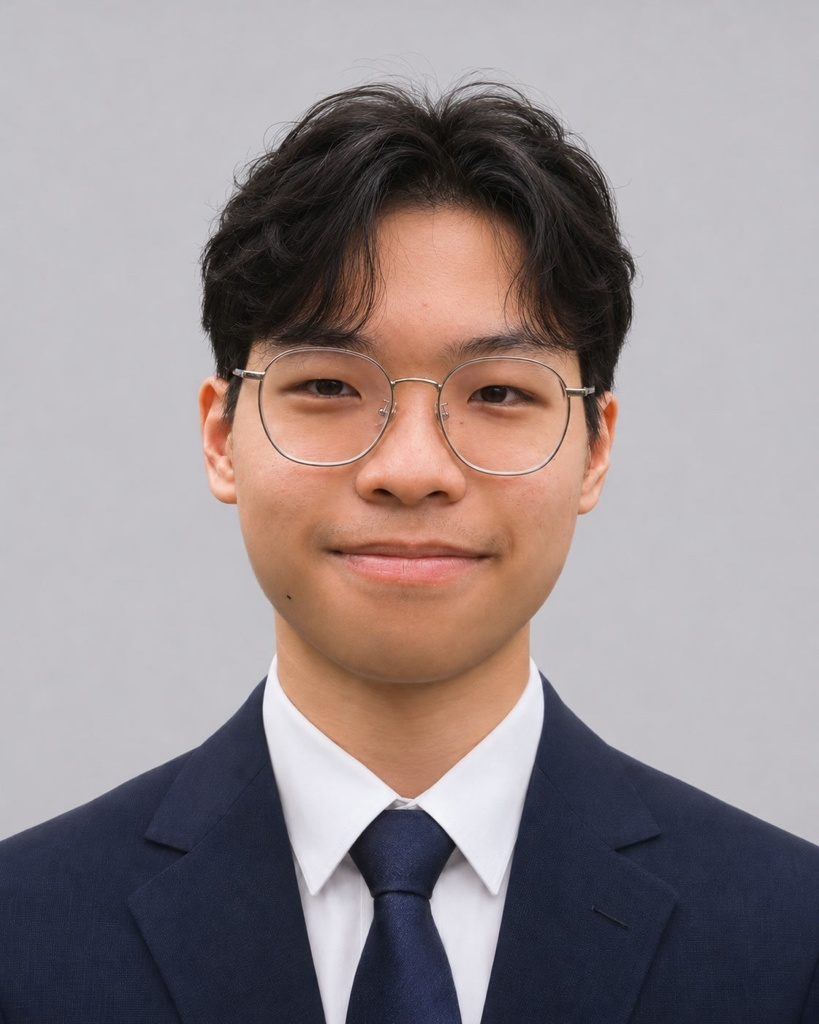
\includegraphics[width=1in,height=1.25in,keepaspectratio,clip]{figures/authors/foo-jin-wayne.jpg}}]{Foo Jin Wayne}
is pursuing a diploma in computer science.

He is with the Research Centre for Human-Machine Collaboration (HUMAC), Faculty of Engineering and Technology, Sunway University, Bandar Sunway, Malaysia. His research focuses on simulated hexapod locomotion and route planning that accounts for individual motor temperatures. He is investigating whether training with deformable soil models improves hexapod walking performance on unfamiliar terrain.
\end{biography}

\begin{biography}[{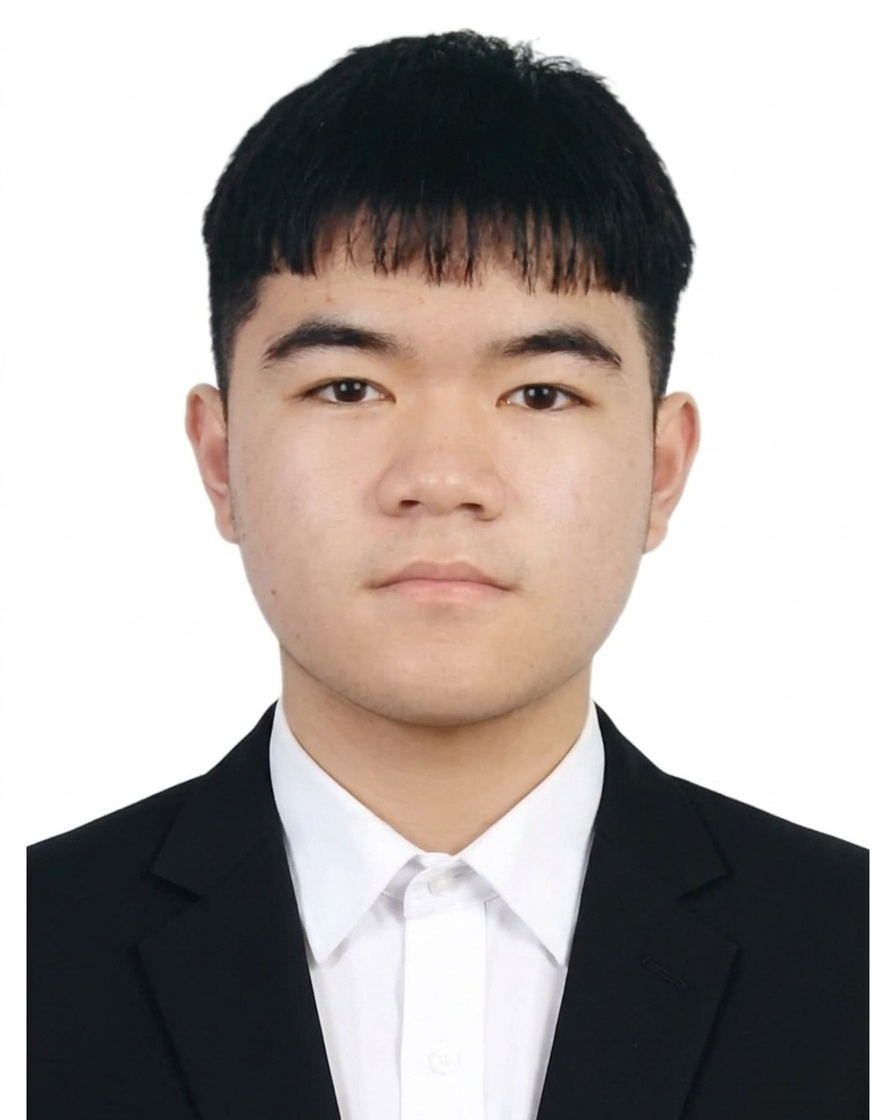
\includegraphics[width=1in,height=1.25in,keepaspectratio,clip]{figures/authors/juo-wei-lai.jpg}}]{Juo Wei Lai}
is affiliated with the research centre for human machine collaboration (HUMAC), Faculty of engineering and Technology, Bandar Sunway, Malaysia [Diploma in Information Technology, Jan 2025]. His research focuses more towards mobile robot navigation, coverage path, and simulation for hexapod inspection applications. Through the project of MINIS, he explores more on mission planning for browser-based, waypoint execution, and synthetic inspection mapping, with an emphasis on system behaviour and reproducible evaluation of simulation results.
\end{biography}

\begin{biography}[{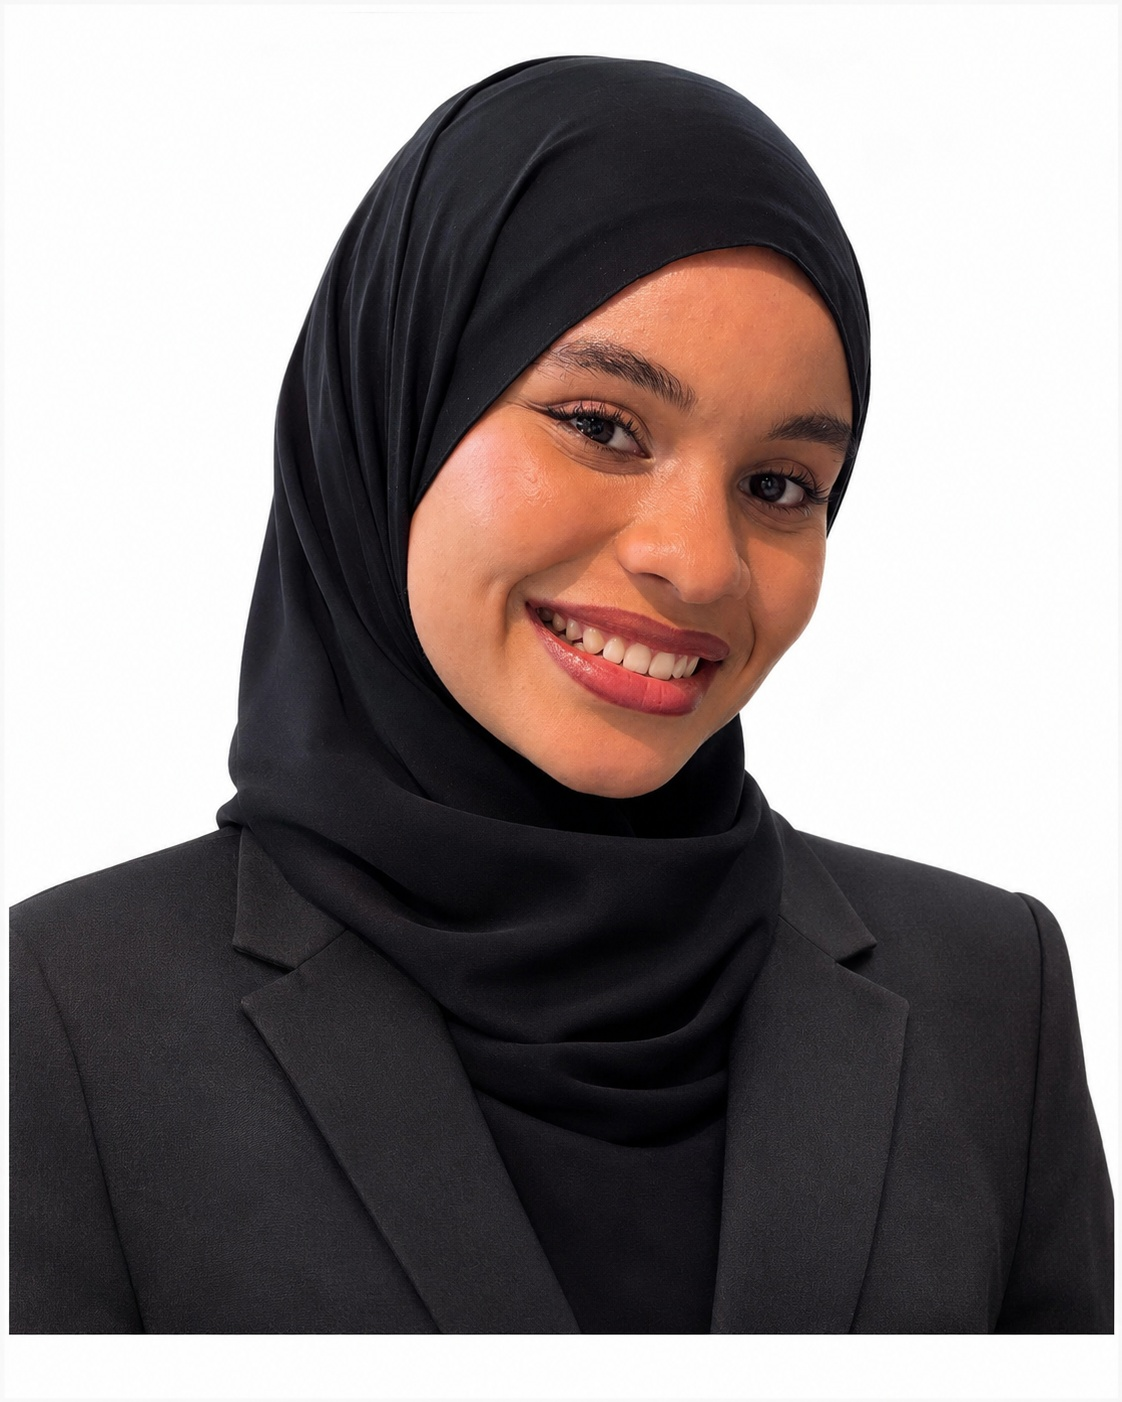
\includegraphics[width=1in,height=1.25in,keepaspectratio,clip]{figures/authors/latifah-mohammed-abdulrahman.jpg}}]{Latifah Mohammed Abdulrahman}
has undertaken diploma studies in computer science.

She is with the Research Centre for Human-Machine Collaboration (HUMAC), Faculty of Engineering and Technology, Sunway University, Bandar Sunway, Malaysia. She studies dynamic jumping on a simulated 18-joint hexapod using central pattern generators, geometric foot steering, landing feedback, and bounded corrections learned through proximal policy optimization. Her work compares residual joint control, oscillator parameter modulation, and direct position control for continuous multihop jumping, directional control, and landing recovery across four jumping stages.
\end{biography}

\begin{biography}[{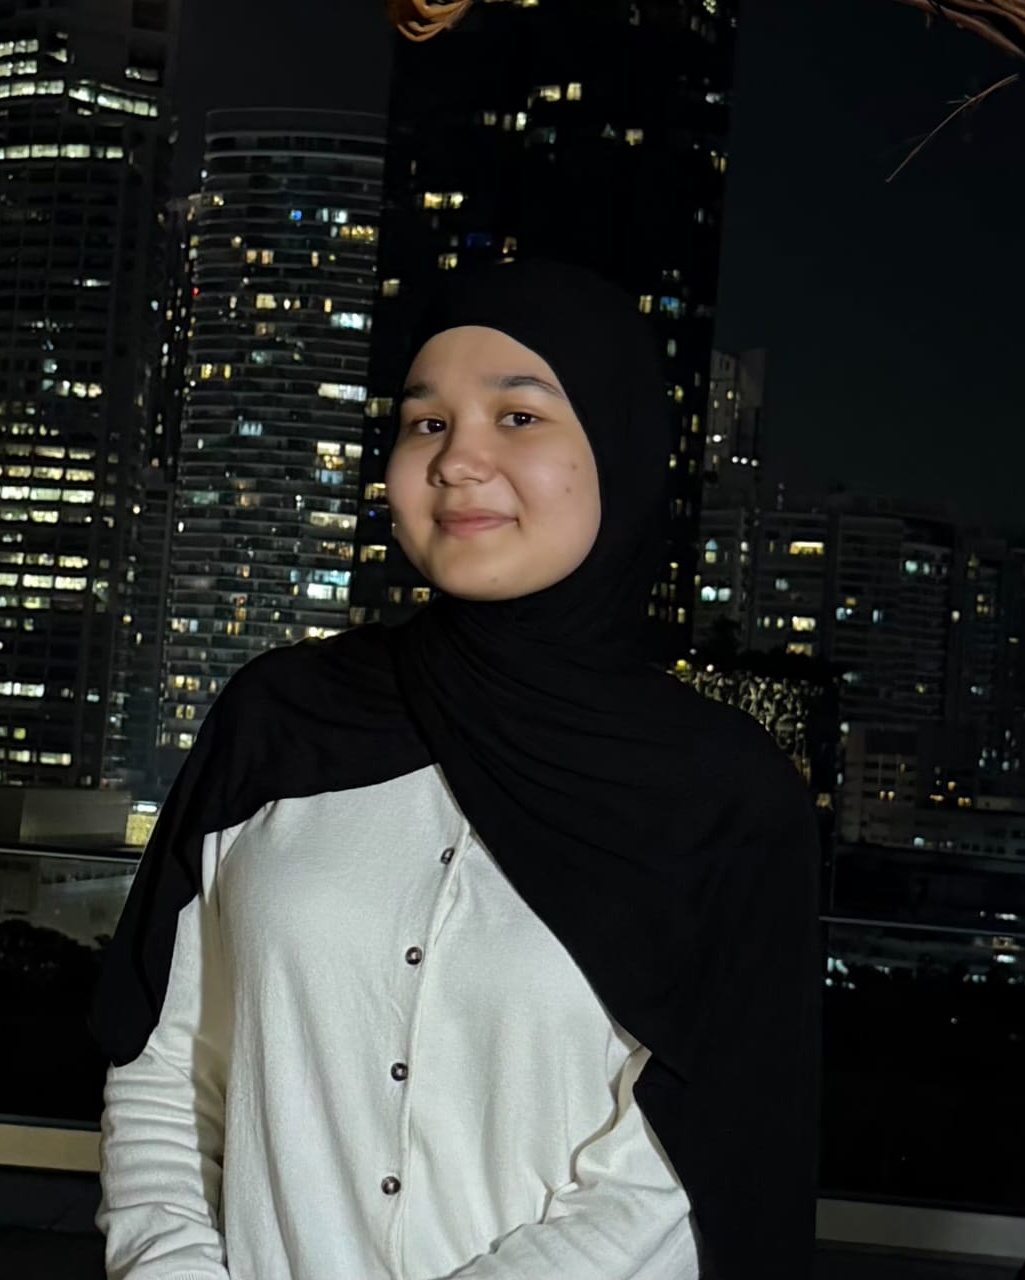
\includegraphics[width=1in,height=1.25in,keepaspectratio,clip]{figures/authors/gulhajar-melebayeva.jpg}}]{Gulhajar Melebayeva}
has undertaken diploma studies in information technology.

She is an intern with the Research Centre for Human-Machine Collaboration (HUMAC), Faculty of Engineering and Technology, Sunway University, Bandar Sunway, Malaysia. Her research combines bioinspired central pattern generators with deep reinforcement learning for multilegged robots. She studies bounded residual reinforcement learning, continuous multistage jumping, and contact recovery, and assesses controller robustness and numerical sensitivity in rigid-body simulations of 18-degree-of-freedom hexapods.
\end{biography}

\begin{biography}[{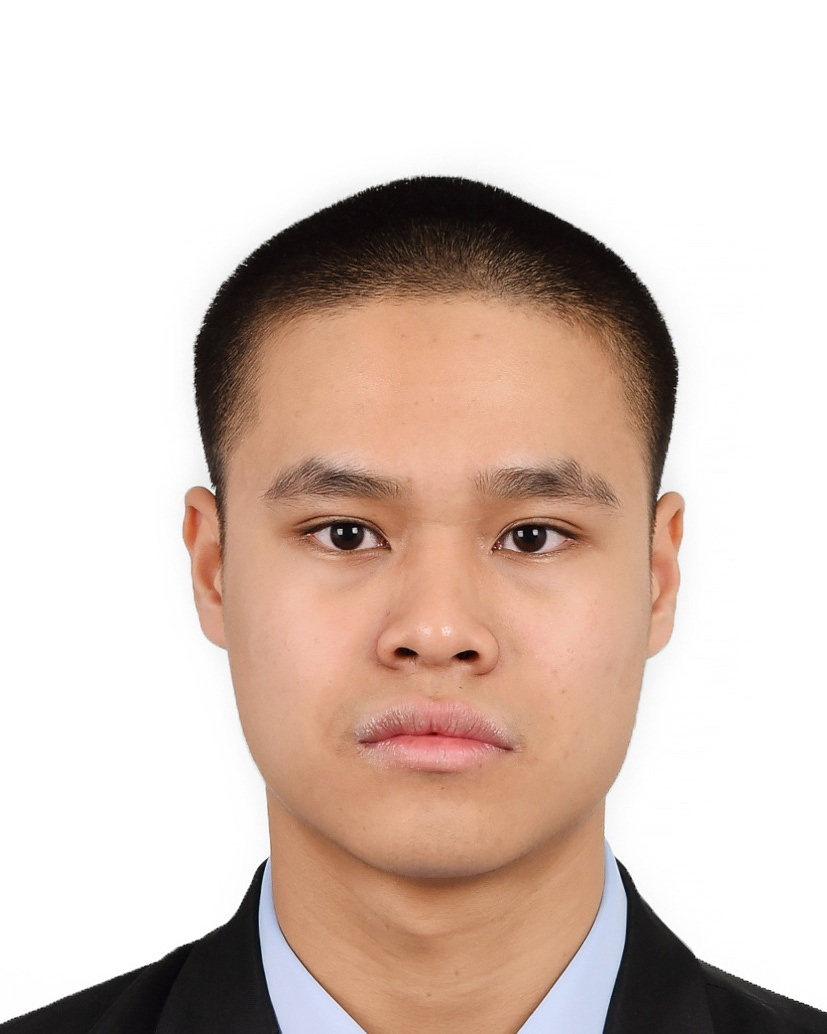
\includegraphics[width=1in,height=1.25in,keepaspectratio,clip]{figures/authors/wen-zer-goo.jpg}}]{Wen Zer Goo}
has undertaken diploma studies in information technology.

He is with the Research Centre for Human-Machine Collaboration (HUMAC), Faculty of Engineering and Technology, Sunway University, Bandar Sunway, Malaysia. His research focuses on visual obstacle perception and vision-language reasoning for simulated hexapod navigation. He has compared a task-trained YOLO detector, a pretrained YOLO-World detector, and a locally run vision-language model across seven obstacle scenarios, examining yielding, bypass behavior, and decision latency with a shared ROS 2 controller and RGB-D sensing.
\end{biography}

\begin{biography}[{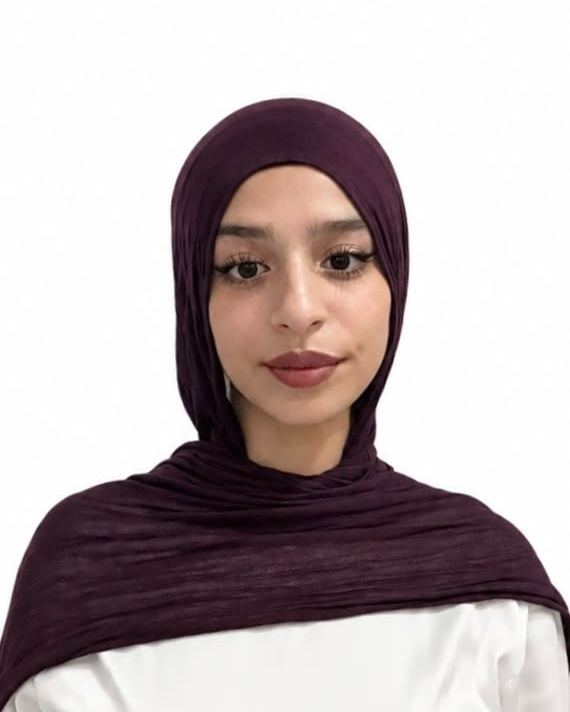
\includegraphics[width=1in,height=1.25in,keepaspectratio,clip]{figures/authors/anfel-fodil.jpg}}]{Anfel Fodil}
has undertaken diploma studies in computer science.

She is with the Research Centre for Human-Machine Collaboration (HUMAC), Faculty of Engineering and Technology, Sunway University, Bandar Sunway, Malaysia. Her research focuses on reinforcement learning and hexapod swimming. She combines proximal policy optimization with central pattern generators in NVIDIA Isaac simulations to study locomotion under mild water currents. She compares learned controllers with conventional central pattern generator baselines using swimming speed, stability, energy efficiency, and heading control.
\end{biography}

\begin{biography}[{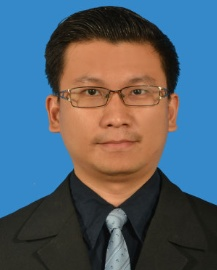
\includegraphics[width=1in,height=1.25in,keepaspectratio,clip]{figures/authors/tiong-yew-tang.jpg}}]{Tiong Yew Tang}
(Member, IEEE) received the bachelor's degree (Hons.) in information system engineering from Universiti Tunku Abdul Rahman in 2006 and the Ph.D. degree in information technology from Monash University in 2016.

He serves on the research committee at Sunway University, Malaysia. He is named as an inventor on a published international patent application filed under the Patent Cooperation Treaty. He works on applications of artificial intelligence in business research. His research interests include bibliometric analysis, artificial intelligence, deep learning, robotic process automation, business intelligence, big data analytics, and computational intelligence.

Dr. Tang received the Book Price Award in 2006 and the Dean's List Award in 2004 and 2005 from Universiti Tunku Abdul Rahman. In 2011, he received the PVC's Award for Excellence in Research, Teaching, and Administration (Round 2) from Monash University.
\end{biography}

\begin{biography}[{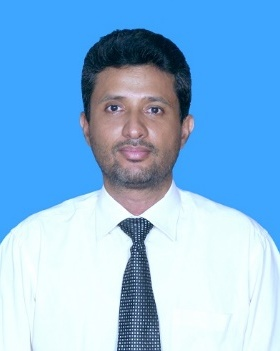
\includegraphics[width=1in,height=1.25in,keepaspectratio,clip]{figures/authors/mohammad-ahmed-alomari.jpg}}]{Mohammad Ahmed Alomari}
(Senior Member, IEEE) received the M.Sc. and Ph.D. degrees in computer systems engineering from Universiti Putra Malaysia, Malaysia.

He is a Senior Lecturer with the Department of Cyber Security, Faculty of Artificial Intelligence and Cyber Security, Universiti Teknikal Malaysia Melaka, Melaka, Malaysia. He has authored and coauthored journal and conference papers. His research interests include mobile data storage encryption, security for smart grids and renewable energy systems, embedded systems, and cryptography. His current work also covers the Internet of Things, blockchain, and cloud computing.

Dr. Alomari is a Professional Technologist registered with the Malaysia Board of Technologists and a member of the International Association of Engineers. He reviews for Springer and SAI journals and serves on organizing and technical committees for conferences and workshops in Malaysia and Japan.
\end{biography}

\begin{biography}[{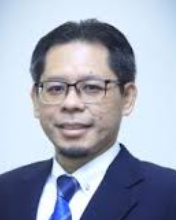
\includegraphics[width=1in,height=1.25in,keepaspectratio,clip]{figures/authors/muhammad-hafidz-fazli-bin-md-fauadi.jpg}}]{Muhammad Hafidz Fazli Bin Md Fauadi}
received the bachelor's degree in industrial computing from Universiti Kebangsaan Malaysia in 2004, the M.Eng. degree in mechanical engineering (advanced manufacturing technology) from Universiti Teknologi Malaysia in 2006, and the D.Eng. degree in information, production, and system engineering from Waseda University, Japan, in 2012.

He is a Professor and the founding Dean of the Faculty of Artificial Intelligence and Cyber Security, Universiti Teknikal Malaysia Melaka, Melaka, Malaysia. His research interests include applied artificial intelligence, system simulation and optimization, intelligent manufacturing systems, cloud manufacturing, and the Internet of Things.

Prof. Muhammad Hafidz Fazli is a Certified HRDF Trainer, a Professional Technologist, and the Chief Editor of the \emph{Journal of Advanced Manufacturing Technology}.
\end{biography}
